\heading{Introduction}
This lab demonstrates the configuration and connectivity of three distinct sites within a company: a main office, a remote branch, and a smart home environment. The setup includes routers, switches, PCs, a server, a wireless home gateway, and IoT devices (light, fan, door). The goal is to establish seamless communication between these sites while ensuring secure and efficient data transfer.


\heading{Objectives}
\begin{enumerate}
   \item To configure routers and the wireless home gateway for inter-site connectivity.
   \item To integrate IoT devices into the network and enable remote control via the server.
   \item To verify end-to-end communication between the main office, remote branch, and smart home environment.
\end{enumerate}


\heading{Model}
\begin{figure}[th]
   \centering
   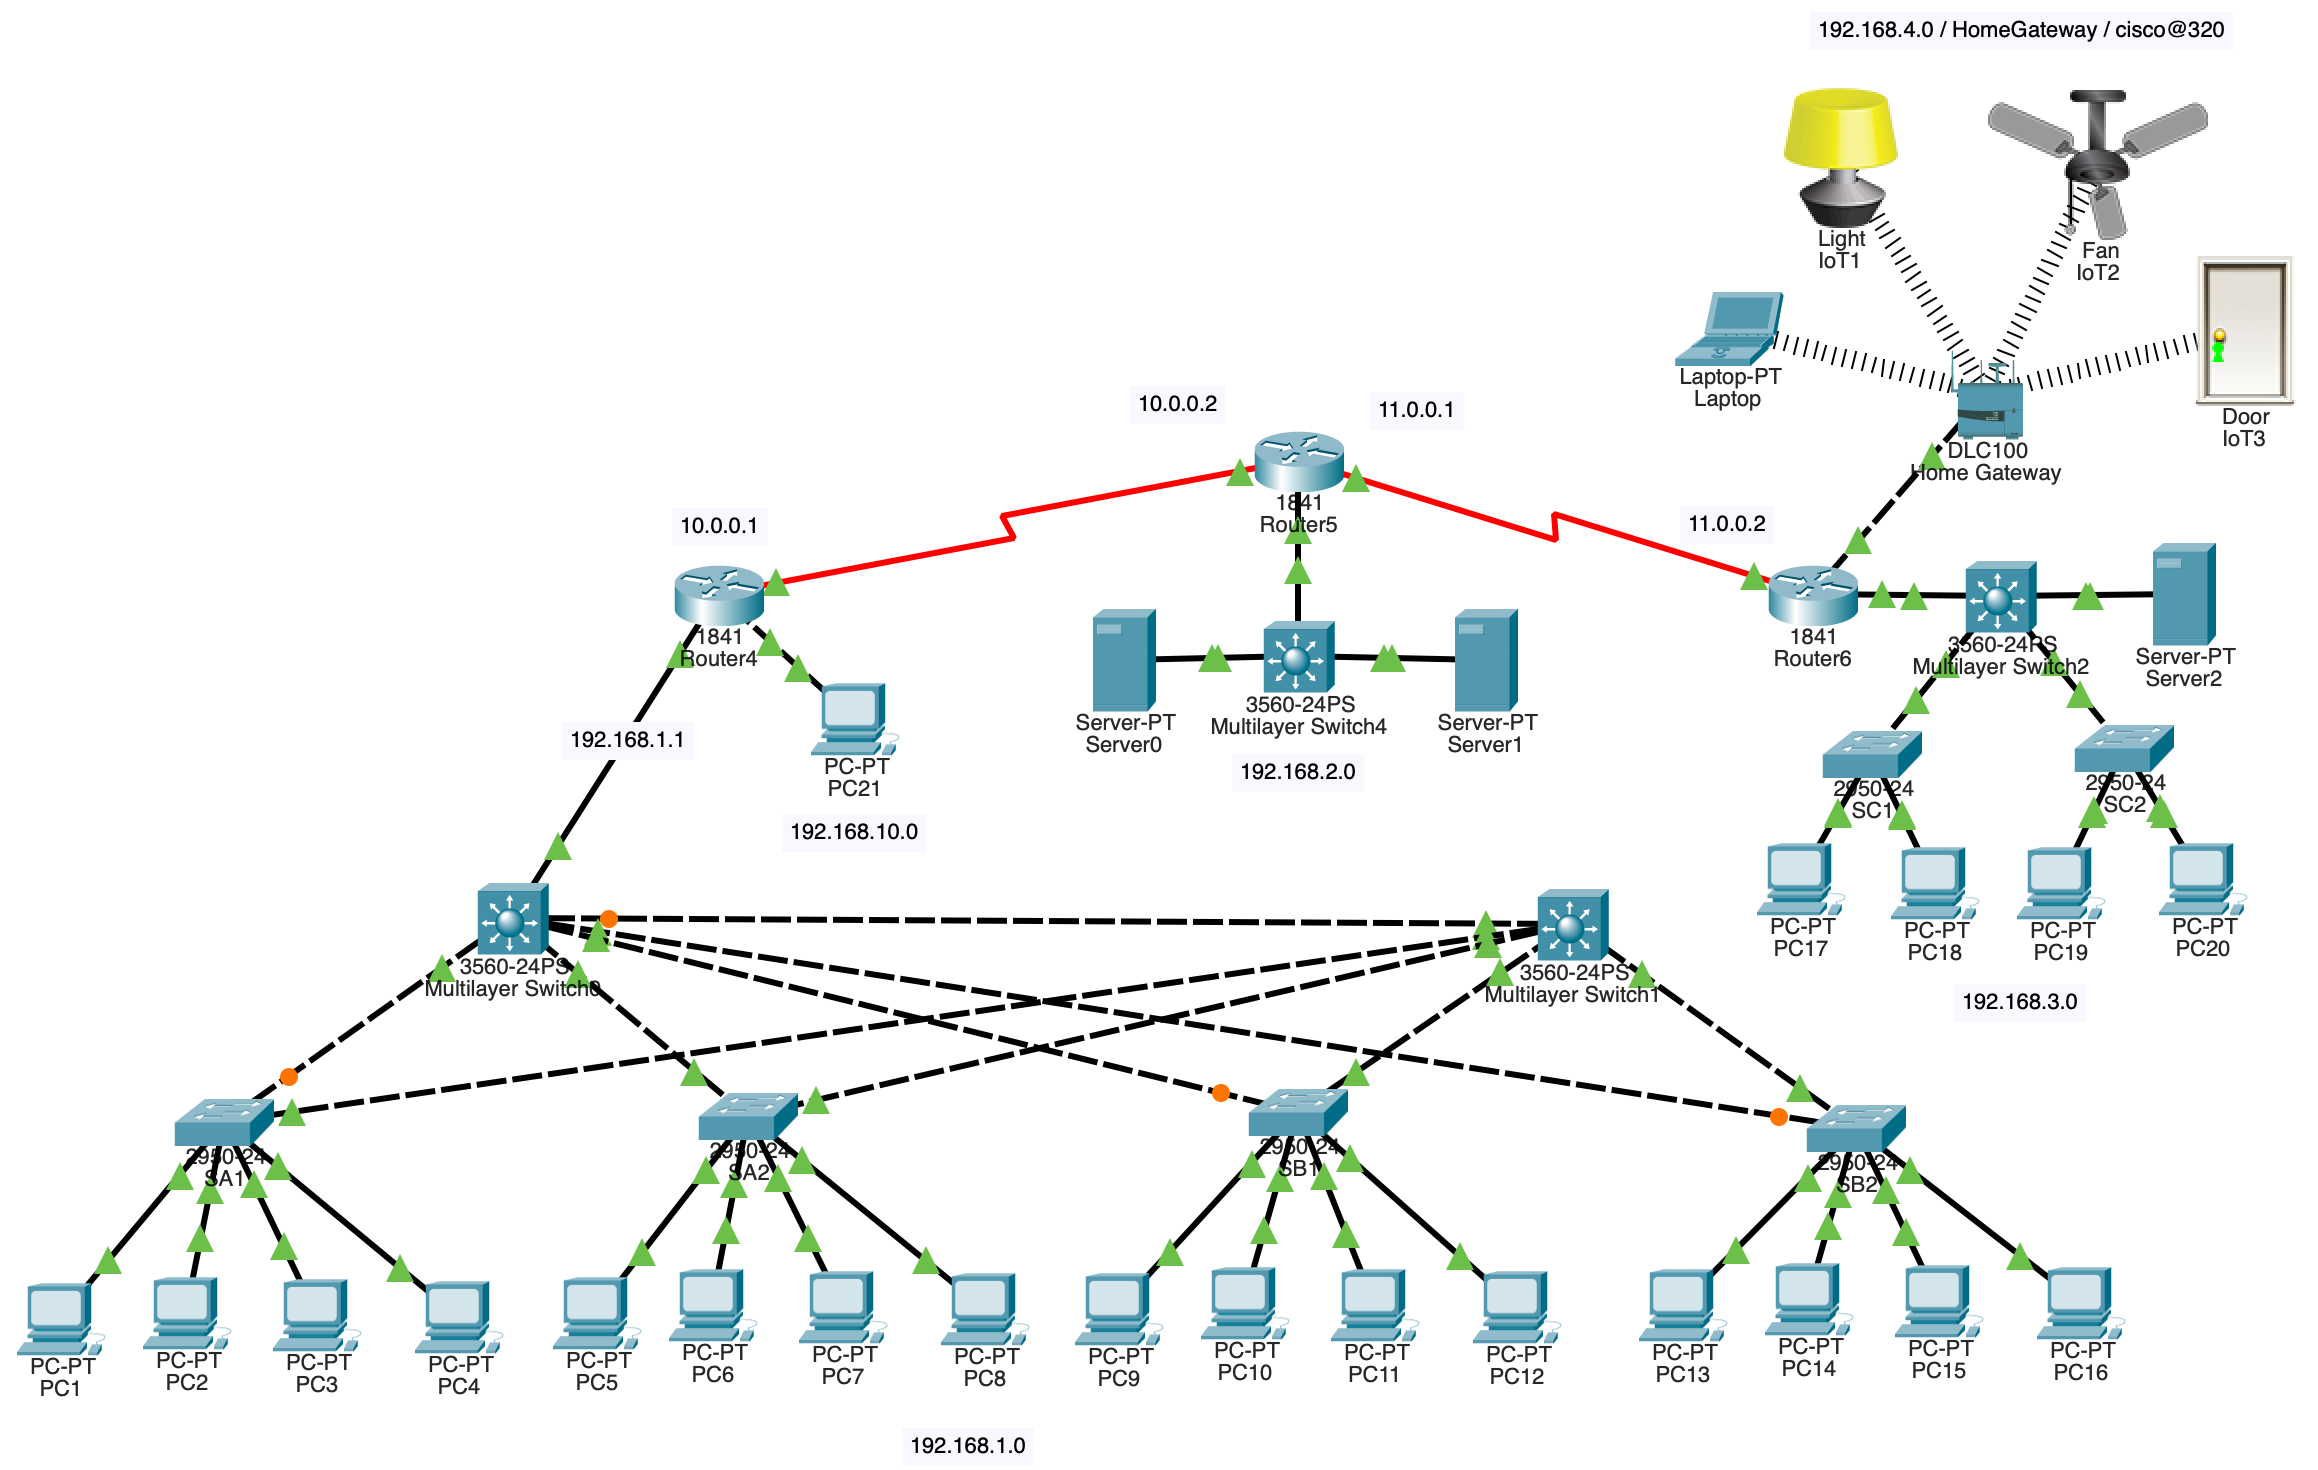
\includegraphics[width=\textwidth]{figures/Exp-1.png}
   \caption{Static IP addressing with 6 PCs, 3 switches, and 3 serially connected routers.}
\end{figure}

\textbf{Model Description}\\
The network model consists of the following components:
\begin{enumerate}[itemsep=1ex]
   \item \textbf{Router}: Used to connect the main office, remote branch, and smart home environment. Routers are configured with static or dynamic routing protocols to ensure data packets are forwarded correctly between sites.

   \item \textbf{Switch}: Connects PCs and the server within the main office and remote branch, enabling local communication within each site.
   
   \item \textbf{Personal Computer (PC)}: Represents user workstations in the main office and remote branch, used for accessing resources and managing the network.
   
   \item \textbf{Server}: Hosts applications and services, such as IoT device management, and acts as a central point for data storage and processing.
   
   \item \textbf{Home Gateway (Wireless)}: Connects IoT devices in the smart home environment to the network, providing wireless access and enabling remote control.
   
   \item \textbf{IoT Devices (Light, Fan, Door)}: Smart devices integrated into the home gateway, allowing remote monitoring and control via the server.
\end{enumerate}

\heading{Pinging Devices \& TTL}
\begin{figure}[th]
   \centering
   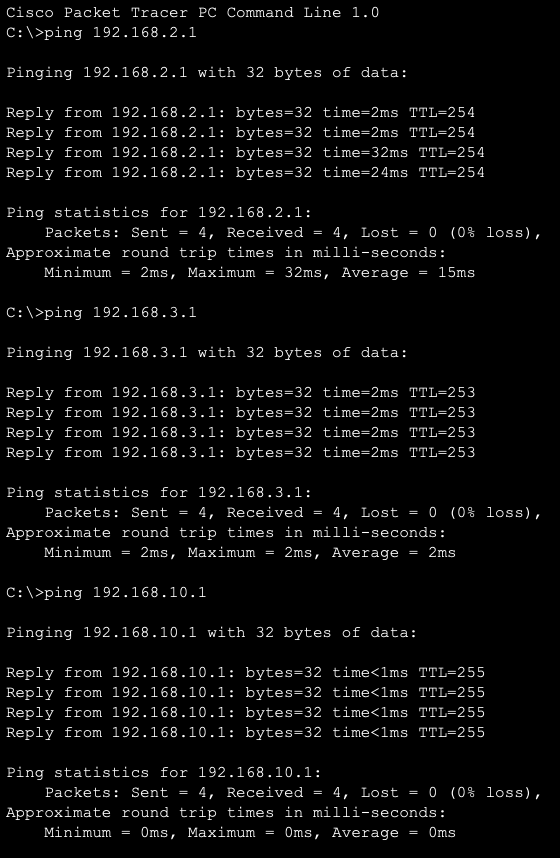
\includegraphics[width=0.7\textwidth]{figures/Exp-1-Ping.png}
   \caption{Pinging other network devices from 192.168.1.4}
\end{figure}

\pagebreak
\heading{Routing Table}
\begin{tabularx}{\textwidth}{XXXX}
\textbf{Device Name} & \textbf{IP Address} &
\textbf{Subnet Mask} & \textbf{Default Gateway}\\
   PC1 & 192.168.1.4 & 255.255.255.0 & 192.168.1.1\\
   PC2 & 192.168.1.5 & 255.255.255.0 & 192.168.1.1\\
   PC3 & 192.168.1.6 & 255.255.255.0 & 192.168.1.1\\
   PC4 & 192.168.1.7 & 255.255.255.0 & 192.168.1.1\\

   PC5 & 192.168.1.8 & 255.255.255.0 & 192.168.1.1\\
   PC6 & 192.168.1.9 & 255.255.255.0 & 192.168.1.1\\
   PC7 & 192.168.1.10 & 255.255.255.0 & 192.168.1.1\\
   PC8 & 192.168.1.11 & 255.255.255.0 & 192.168.1.1\\

   PC9 & 192.168.1.12 & 255.255.255.0 & 192.168.1.1\\
   PC10 & 192.168.1.13 & 255.255.255.0 & 192.168.1.1\\
   PC11 & 192.168.1.14 & 255.255.255.0 & 192.168.1.1\\
   PC12 & 192.168.1.15 & 255.255.255.0 & 192.168.1.1\\

   PC13 & 192.168.1.16 & 255.255.255.0 & 192.168.1.1\\
   PC14 & 192.168.1.17 & 255.255.255.0 & 192.168.1.1\\
   PC15 & 192.168.1.18 & 255.255.255.0 & 192.168.1.1\\
   PC16 & 192.168.1.19 & 255.255.255.0 & 192.168.1.1\\

   PC17 & 192.168.3.2 & 255.255.255.0 & 192.168.3.1\\
   PC18 & 192.168.3.3 & 255.255.255.0 & 192.168.3.1\\
   PC19 & 192.168.3.4 & 255.255.255.0 & 192.168.3.1\\
   PC20 & 192.168.3.5 & 255.255.255.0 & 192.168.3.1\\
   
   PC21 & 192.168.10.2 & 255.255.255.0 & 192.168.10.1\\
   
   Server0 & 192.168.2.2 & 255.255.255.0 & 192.168.2.1\\
   Server1 & 192.168.2.3 & 255.255.255.0 & 192.168.2.1\\
   Server2 & 192.168.3.6 & 255.255.255.0 & 192.168.3.1\\

   
   Router1 (s/0/0) & 10.0.0.1 & 255.0.0.0\\
   Router2 (s/0/0) & 10.0.0.2 & 255.0.0.0\\
   Router2 (s/0/1) & 11.0.0.1 & 255.0.0.0\\
   Router3 (s/0/0) & 11.0.0.2 & 255.0.0.0\\\\

   Home Gateway & SSID: HomeGateway & WPA2-PSK: cisco@320 \\
   Light, Fan, Door & DHCP
\end{tabularx}



\pagebreak
\heading{Complexity}
The lab involves configuring multiple network devices across different sites, which requires careful planning of IP addressing, routing, and security policies. Integrating IoT devices adds another layer of complexity, as they must be securely connected to the network and configured for remote access. Ensuring seamless communication between the main office, remote branch, and smart home environment requires thorough testing and troubleshooting.

\heading{Discussion}
The lab successfully demonstrated the connection of three different company sites using routers, a server, and a wireless home gateway. IoT devices were integrated into the network and controlled remotely via the server, showcasing the potential of smart environments in a corporate setting. The exercise highlighted the importance of proper configuration and security measures in multi-site networks, ensuring reliable and secure communication across all locations.